\documentclass[11pt]{article}
\usepackage[scaled=0.92]{helvet}
\usepackage{geometry}
\geometry{letterpaper,tmargin=1in,bmargin=1in,lmargin=1in,rmargin=1in}
\usepackage[parfill]{parskip} % Activate to begin paragraphs with an empty line rather than an indent %\usepackage{graphicx}
\usepackage{amsmath,amssymb, mathrsfs, dsfont}
\usepackage{mathtools}

\usepackage{tabularx}
\usepackage[font=footnotesize,labelfont=bf]{caption}
\usepackage{graphicx}
\usepackage{xcolor}
%\usepackage[linkbordercolor ={1 1 1} ]{hyperref}
%\usepackage[sf]{titlesec}
\usepackage{natbib}
\usepackage{../../Tianpei_Report}

%\usepackage{appendix}
%\usepackage{algorithm}
%\usepackage{algorithmic}

%\renewcommand{\algorithmicrequire}{\textbf{Input:}}
%\renewcommand{\algorithmicensure}{\textbf{Output:}}



\begin{document}
\title{Lecture 10: Policy Gradient Methods}
\author{Tianpei Xie}
\date{ Aug 13th., 2022 }
\maketitle
\tableofcontents
\newpage
\section{Value-based methods vs. Policy-based methods}
By far, we mainly discussed the value-based methods, this chapter, we focus on policy-based methods. 
\begin{itemize}
\item \textbf{Value-based methods} (or \emph{action-value methods}): all these methods (DP, MC, TD with tabular or function approximation) learned the \textbf{values of actions} and then \underline{selected actions} based on their estimated action values; their policies would not even exist without the action-value estimates.

\item \textbf{Policy-based methods} (or \emph{policy gradient methods}): methods that instead learn a \textbf{parameterized policy} that can select actions \emph{without consulting} a value function.  A \emph{value}
function may still be used to \underline{\emph{learn the policy parameter}}, but is not required for action selection. 

Perhaps the simplest \textbf{advantage} that \textbf{policy parameterization} may have over \textbf{action-value parameterization} is that the policy may be a simpler function to approximate. Problems vary in the complexity of their policies and action-value functions. 


Finally, we note that the choice of policy parameterization is sometimes a good way of \textbf{injecting prior knowledge} about the desired form of the policy into the reinforcement learning system. This is often the most important reason for using a policy-based learning method.
\end{itemize}

Denote $\mb{\theta} \in \bR^{m}$, the parameterized policy distribution over $a \in \cA(s)$ at time $t$ is $\pi(a |\mb{s}, \mb{\theta}) := Pr\{A_t =a | S_{t}=\mb{s}, \mb{\theta}_t=\mb{\theta}\}$. The \emph{goal} of policy optimization is to find policy $\pi$ that \emph{\textbf{maximizes}} some \textbf{objective function} $\cR(\mb{\theta}_t)$. For instance, for continuing tasks with ergodic MDP, we choose \textbf{average rewards} $\cR(\mb{\theta}_t) := r(\pi(a |\mb{s}, \mb{\theta}))$
\begin{align}
r(\pi(a |\mb{s}, \mb{\theta})) &= \sum_{s}\mu_{\pi}(s)\sum_{a}\pi(a |s, \mb{\theta}) \sum_{s', r}p(s', r| s, a)r.  \label{eqn: avg_reward_discount_continuing3}
\end{align}

\subsection{Policy Gradient methods}
In order to optimize the objective function \eqref{eqn: avg_reward_discount_continuing3}, we use the \emph{gradient acsent algorithm}
\begin{align}
\mb{\theta}_{t+1} &\leftarrow \mb{\theta}_t + \alpha \grad{\mb{\theta}}{\widehat{\cR(\mb{\theta}_t)}}. \label{eqn: grad_ascent}
\end{align} All methods that follow the general schema \eqref{eqn: grad_ascent} we call \textbf{\emph{policy gradient methods}}, whether or not they also learn an approximate value function. Methods that learn approximations to \emph{both policy and value functions} are often called \textbf{\emph{actor-critic methods}}, where '\emph{\textbf{actor}}' is a reference to the \underline{learned policy}, and '\textbf{\emph{critic}}' refers to the \underline{learned value function}, usually a state-value function.

\section{Policy approximation}
Depending on if the action space  $\cA$ is finite discrete or continous, we can approximate the paremeterized policy distribution using different functions:
\begin{itemize}
\item When $\cA$ is \textbf{finite discrete}, and $\mb{s} \in \cS$, we can ues the \textbf{soft-max function} to approximate the policy function
\begin{align}
\pi(a |\mb{s}, \mb{\theta}) &= \frac{\exp\paren{h(\mb{s}, a, \mb{\theta})}}{\sum_{a'}\exp\paren{h(\mb{s}, a', \mb{\theta})}} \label{eqn: soft_max_policy} \\
\log \pi(a |\mb{s}, \mb{\theta}) &= h(\mb{s}, a, \mb{\theta}) -  \underline{\log \sum_{a'}\exp\paren{h(\mb{s}, a', \mb{\theta})}}  \label{eqn: log_soft_max_policy} \\
\grad{\mb{\theta}}{\log \pi(a |\mb{s}, \mb{\theta}) } &= \grad{\mb{\theta}}{h(\mb{s}, a, \mb{\theta})} - \underline{\E{\pi(a |\mb{s}, \mb{\theta}) }{ \grad{\mb{\theta}}{h(\mb{s}, a, \mb{\theta})}}}   \label{eqn: grad_log_soft_max_policy} \\
&= \grad{\mb{\theta}}{h(\mb{s}, a, \mb{\theta})} - \sum_{a'}\pi(a' |\mb{s}, \mb{\theta}) \grad{\mb{\theta}}{h(\mb{s}, a', \mb{\theta})} \nonumber\\
&= \text{\textbf{sample} }\grad{\mb{\theta}}{h(\mb{s}, a, \mb{\theta})}\text{ with action} -  \text{\textbf{policy action mean} of }\grad{\mb{\theta}}{h(\mb{s}, a, \mb{\theta})} \nonumber
\end{align} The function $h(\mb{s}, a, \mb{\theta})$ defines the \textbf{preferences} of some actions. This kind of policy parameterization is called  \emph{\textbf{soft-max in action preferences}}. We can define the preference as \emph{linear functions} with respect to some features:
\begin{align*}
h(\mb{s}, a, \mb{\theta}) &:= \inn{\mb{\theta}}{\mb{\phi}(\mb{s}, a)} \\
\grad{\mb{\theta}}{h(\mb{s}, a, \mb{\theta})} &= \mb{\phi}(\mb{s}, a)
\end{align*} where $\mb{\phi}(\mb{s}, a):= [\phi_{k}(\mb{s}, a)]$ can be any feature representation we discussed in lecture 8, for instance, \emph{tile coding} on state on fixed action and stacked multiple actions. Combining with \eqref{eqn: grad_log_soft_max_policy}, we can see that  the gradient of log of $\pi$ can be easily represented as the \textbf{difference} between the \emph{\textbf{\underline{sample (mean)}} of state-action feature} for specific action $\mb{\phi}(\mb{s}, a)$ and \emph{the \textbf{\underline{policy mean}} of state-action feature over all actions} $ \E{\pi(a |\mb{s}, \mb{\theta}) }{ \mb{\phi}(\mb{s}, a)}$.

\begin{itemize}
\item One \textbf{advantage} of parameterizing policies according to the soft-max in action preferences is that the \textbf{\underline{approximate policy can approach a deterministic policy}}, whereas with $\epsilon$-greedy action selection over action values there is always an $\epsilon$ probability of selecting a random action. Of course, one could \emph{\textbf{select} according to a \textbf{soft-max distribution}} based on action values, but this alone would not allow the policy to approach a \textbf{deterministic policy}. Instead, the \textbf{action-value estimates} would converge to their corresponding \textbf{true values}, which would \emph{differ by a finite amount}, translating to specific probabilities other than $0$ and $1$. \textbf{Action preferences} are different because they do not approach specific values; instead they are driven to produce the \emph{\textbf{optimal stochastic policy}}. If the optimal policy is \emph{\textbf{deterministic}}, then the preferences of the optimal actions will be driven infinitely higher than all suboptimal actions (if permitted by the parameterization).

\item A second \textbf{advantage} of parameterizing policies according to the soft-max in action preferences is that it enables the selection of actions with \textbf{arbitrary probabilities}. In problems with significant function approximation, the \textbf{best approximate policy} may be \textbf{stochastic}. For example, in card games with imperfect information the optimal play is often to do two different things with specific probabilities, such as when bluffng in Poker. Action-value methods have no natural way of finding stochastic optimal policies, whereas policy approximating methods can. 
\end{itemize}


\item  When $\cA \subset \bR^{k}$ is \textbf{continuous space},  and $\mb{s} \in \cS$, $\mb{\theta} = [\mb{\theta}_{\mu}, \mb{\theta}_{\sigma}]$
\begin{align}
\pi(a |\mb{s}, \mb{\theta}) &= \frac{1}{\sqrt{2\pi}\sigma(\mb{s}, \mb{\theta}_{\sigma})}\exp\paren{-\frac{(a - \mu(\mb{s}, \mb{\theta}_{\mu}))^2}{2\sigma(\mb{s}, \mb{\theta}_{\sigma})^2}}
 \label{eqn: normal_policy} \\
\log \pi(a |\mb{s}, \mb{\theta}) &= -\frac{(a - \mu(\mb{s}, \mb{\theta}_{\mu}) )^2}{2\sigma(\mb{s}, \mb{\theta}_{\sigma})^2} - \log\sigma(\mb{s}, \mb{\theta}_{\sigma})+ \frac{1}{2}\log{2\pi} \label{eqn: log_normal_policy} \\
\grad{\mb{\theta}}{\log \pi(a |\mb{s}, \mb{\theta}) } &= \grad{\mb{\theta}}{h(\mb{s}, a, \mb{\theta})} - \underline{\E{\pi(a |\mb{s}, \mb{\theta}) }{ \grad{\mb{\theta}}{h(\mb{s}, a, \mb{\theta})}}}   \label{eqn: grad_log_normal_policy} \\
&= \text{\textbf{sample} of }\grad{\mb{\theta}}{h(\mb{s}, a, \mb{\theta})} -  \text{\textbf{policy action mean} of }\grad{\mb{\theta}}{h(\mb{s}, a, \mb{\theta})} \nonumber
\end{align} where 
\begin{align*}
h(\mb{s}, a,\mb{\theta}) &= -\frac{(a - \mu(\mb{s}, \mb{\theta}_{\mu}))^2}{2\sigma(\mb{s}, \mb{\theta}_{\sigma})^2}\\
\mu(\mb{s}, \mb{\theta}_{\mu}) &= \inn{\mb{\theta}_{\mu}}{\mb{\phi}_{\mu}(\mb{s})} \\
\sigma(\mb{s}, \mb{\theta}_{\sigma}) &= \exp(\inn{\mb{\theta}_{\sigma}}{\mb{\phi}_{\sigma}(\mb{s})})
\end{align*}
Note that
\begin{align*}
\grad{\mb{\theta}_{\mu}}{\log \pi(a |\mb{s}, \mb{\theta}) } &= \frac{1}{\sigma(\mb{s}, \mb{\theta}_{\sigma})^2}\paren{a - \mu(\mb{s}, \mb{\theta}_{\mu})}\grad{\mb{\theta}_{\mu}}{\mu(\mb{s}, \mb{\theta}_{\mu}) } \\
&= \frac{1}{\sigma(\mb{s}, \mb{\theta}_{\sigma})^2}\paren{a - \mu(\mb{s}, \mb{\theta}_{\mu})}\mb{\phi}_{\mu}(\mb{s}) \\
\grad{\mb{\theta}_{\sigma}}{\log \pi(a |\mb{s}, \mb{\theta}) } &=(a - \mu(\mb{s}, \mb{\theta}_{\mu}))^2 \frac{1}{\sigma(\mb{s}, \mb{\theta}_{\sigma})^3}\grad{\mb{\theta}_{\sigma}}{\sigma(\mb{s}, \mb{\theta}_{\sigma}) } - \frac{1}{\sigma(\mb{s}, \mb{\theta}_{\sigma})}\grad{\mb{\theta}_{\sigma}}{\sigma(\mb{s}, \mb{\theta}_{\sigma}) } \\
&= \paren{\frac{(a - \mu(\mb{s}, \mb{\theta}_{\mu}))^2-\sigma(\mb{s}, \mb{\theta}_{\sigma})^2}{\sigma(\mb{s}, \mb{\theta}_{\sigma})^3}}\grad{\mb{\theta}_{\sigma}}{\sigma(\mb{s}, \mb{\theta}_{\sigma}) } \\
&= \paren{\frac{(a - \mu(\mb{s}, \mb{\theta}_{\mu}))^2-\sigma(\mb{s}, \mb{\theta}_{\sigma})^2}{\sigma(\mb{s}, \mb{\theta}_{\sigma})^3}}\sigma(\mb{s}, \mb{\theta}_{\sigma})\mb{\phi}_{\sigma}(\mb{s}) \\
&= \paren{\frac{(a - \mu(\mb{s}, \mb{\theta}_{\mu}))^2}{\sigma(\mb{s}, \mb{\theta}_{\sigma})^2} - 1}\mb{\phi}_{\sigma}(\mb{s})
\end{align*}
\end{itemize}

\section{The Policy Gradient Theorem}
With continuous policy parameterization the action probabilities \textbf{change smoothly} as a function of the learned parameter, whereas in $\epsilon$-greedy selection the action probabilities may change dramatically for an arbitrarily small change in the estimated action values, if that change results in a different action having the maximal value.  Largely because of this \textbf{stronger convergence guarantees} are available for \underline{policy-gradient methods} than for action-value methods.

The objective function $\cR(\mb{\theta})$ for episodic and continuing tasks are different.
\begin{itemize}
\item For \textbf{episodic task}, the objective function is the expected returns i.e. the value function under policy $\pi$ of the start state of the episode:
\begin{align}
\cR(\mb{\theta}) &:= v_{\pi( \mb{\theta})}(\mb{s}_{0})  \nonumber\\
&=\sum_{a}\pi(a |\mb{s}_{0}, \mb{\theta})q_{\pi}(\mb{s}_{0}, a)  \label{eqn: obj_policy_grad_episodic}
\end{align}

\item For \textbf{continuing task}, the objective function is the average rewards
\begin{align}
\cR(\mb{\theta}) &:= r(\pi(a |\mb{s}, \mb{\theta}))  \nonumber \\
&= \sum_{s}\mu_{\pi(\mb{\theta})}(s)\sum_{a}\pi(a |s, \mb{\theta}) \sum_{s', r}p(s', r| s, a)r.  \label{eqn: obj_policy_grad_continuing}
\end{align} where $\mb{\mu}$ is the \textbf{steady-state distribution}. It is also called the \textbf{limiting state distribution} under $\pi$, $\mu(s) = \lim_{t\rightarrow \infty}Pr\{S_{t} = s| S_{0}, \pi\}$, or \textbf{on-policy distribution} under policy $\pi$.
\end{itemize}


With function approximation, it may seem challenging to change the \emph{policy} parameter in a way that ensures \textbf{improvement}. The problem is that performance depends on both the \textbf{action selections} and the \textbf{distribution of states} in which those selections are made, and that \emph{both of these are affected by the policy} parameter. Note that the effect of the policy on the \underline{state distribution} $\mb{\mu}(s)$ is a function of the environment and is typically unknown.

Fortunately, there is an excellent theoretical answer to this challenge in the form of the \textbf{policy gradient theorem}, which provides an analytic expression for the gradient of performance with respect to the policy parameter (which is what we need to approximate for gradient ascent) that \textbf{does not involve the derivative of the state distribution}.

\begin{theorem} (\textbf{Policy gradient theorem})
For both the episodic case and continuing case under ergodic MDP, the objective functions $\cR(\mb{\theta})$ are defined as in \eqref{eqn: obj_policy_grad_episodic} and \eqref{eqn: obj_policy_grad_continuing} respectively. Then 
\begin{align}
\grad{\mb{\theta}}{\cR(\mb{\theta})} &\propto \sum_{s}\mu_{\pi(\mb{\theta})}(s)\sum_{a}\grad{\mb{\theta}}{\pi(a |\mb{s}, \mb{\theta})}q_{\pi}(\mb{s}, a) \label{eqn: policy_grad_theorem}\\
&= \E{\mb{s} \sim \mb{\mu}_{\pi(\mb{\theta})}}{\sum_{a}\grad{\mb{\theta}}{\pi(a |\mb{s}, \mb{\theta})}q_{\pi}(\mb{s}, a) } \label{eqn: policy_grad_theorem2} \\
&= \E{\mb{s} \sim \mb{\mu}_{\pi(\mb{\theta})}}{\E{a \sim \pi(a|\mb{s}, \mb{\theta})}{\grad{\mb{\theta}}{\log \pi(a |\mb{s}, \mb{\theta})}q_{\pi}(\mb{s}, a) }},\label{eqn: policy_grad_theorem3}
\end{align} where $\mb{\mu}_{\pi}$ is the limiting state distribution under $\pi$, $\mu(s) = \lim_{t\rightarrow \infty}Pr\{S_{t} = s| S_{0}, \pi\}$, (or on-policy distribution under policy $\pi$).  In particular, the gradient of objective does not depend on the gradient of state distribution $\grad{}{\mb{\mu}}$.  For ergodic MDP with average reward objective, the equation \eqref{eqn: policy_grad_theorem} is exact. For episodic task, the constant of proportionality is the average length of an episode.
\end{theorem}
\begin{proof} We prove the case for the continuing task with ergodic MDP. For the episodic task, please refer the book \citep{sutton2018reinforcement} chapter 13.2. We check on the definition of state-value function 
\begin{align*}
v_{\pi}(s) &= \sum_{a}\pi(a|\mb{s}, \mb{\theta})q_{\pi}(s, a) \\
\grad{\mb{\theta}}{v_{\pi}(s) } &= \sum_{a}\grad{\mb{\theta}}{\pi(a|\mb{s}, \mb{\theta})}q_{\pi}(s, a)  +  \sum_{a}\pi(a|\mb{s}, \mb{\theta})\grad{\mb{\theta}}{q_{\pi}(s, a)} \\
&\text{ due to }q_{\pi}(s, a) = \sum_{s', r}p(s', r| s, a)\brac{r- r(\pi) + v_{\pi}(s')}\\
&=  \sum_{a}\grad{\mb{\theta}}{\pi(a|\mb{s}, \mb{\theta})}q_{\pi}(s, a) +  \\
& \sum_{a}\pi(a|\mb{s}, \mb{\theta})\grad{\mb{\theta}}{\sum_{s', r}p(s', r| s, a)\brac{r- r(\pi) + v_{\pi}(s')}}\\
&=  \sum_{a}\grad{\mb{\theta}}{\pi(a|\mb{s}, \mb{\theta})}q_{\pi}(s, a)  + \\
& \sum_{a}\pi(a|\mb{s}, \mb{\theta})\sum_{s', r}p(s', r| s, a)\brac{- \grad{\mb{\theta}}{r(\pi)} + \grad{\mb{\theta}}{v_{\pi}(s')}} 
\end{align*} Rearrange this equation and note that $(\sum_{a}\pi(a|\mb{s}, \mb{\theta}))(\sum_{s', r}p(s', r| s, a)) = 1$:
\begin{align}
\grad{\mb{\theta}}{\cR}:=\grad{\mb{\theta}}{r(\pi)}&= -\grad{\mb{\theta}}{v_{\pi}(s)} + \sum_{a}\brac{\grad{\mb{\theta}}{\pi(a|\mb{s}, \mb{\theta})}q_{\pi}(s, a)  + \pi(a|\mb{s}, \mb{\theta})\sum_{s', r}p(s', r| s, a) \grad{\mb{\theta}}{v_{\pi}(s')}} \label{eqn: grad_avg_rewards}
\end{align} Now note that  left hand side of \eqref{eqn: grad_avg_rewards} is not function of state $\mb{s}$ since the average reward does not depend on state. Therefore the right hand side of \eqref{eqn: grad_avg_rewards} is not a function of  $\mb{s}$ either. Since $\sum_{s}\mu_{\pi(\mb{\theta})}(s) = 1$, we can mulitple both sides $\sum_{s}\mu_{\pi(\mb{\theta})}(s)$:
\begin{align*}
\grad{\mb{\theta}}{\cR} &= \sum_{s}\mu_{\pi}(s)\set{ -\grad{\mb{\theta}}{v_{\pi}(s)} + \sum_{a}\brac{\grad{\mb{\theta}}{\pi(a|\mb{s}, \mb{\theta})}q_{\pi}(s, a)  + \pi(a|\mb{s}, \mb{\theta})\sum_{s', r}p(s', r| s, a) \grad{\mb{\theta}}{v_{\pi}(s')}}} \\
&=  \sum_{s}\mu_{\pi}(s)\sum_{a}\grad{\mb{\theta}}{\pi(a|\mb{s}, \mb{\theta})}q_{\pi}(s, a) +
\sum_{s}\mu_{\pi}(s)\set{ -\grad{\mb{\theta}}{v_{\pi}(s)} +\sum_{a}\pi(a|\mb{s}, \mb{\theta})\sum_{s', r}p(s', r| s, a) \grad{\mb{\theta}}{v_{\pi}(s')}}\\
&=  \sum_{s}\mu_{\pi}(s)\sum_{a}\grad{\mb{\theta}}{\pi(a|\mb{s}, \mb{\theta})}q_{\pi}(s, a) - \sum_{s}\mu_{\pi}(s) \grad{\mb{\theta}}{v_{\pi}(s)}  + \\
& \sum_{s'}\paren{\sum_{s}\mu_{\pi}(s)\sum_{a}\pi(a|\mb{s}, \mb{\theta})\sum_{r}p(s', r| s, a)} \grad{\mb{\theta}}{v_{\pi}(s')}
\end{align*}
Recall  that the steady-state distribution $\mb{\mu}$ has the following equation
\begin{align*}
\sum_{s}\mu_{\pi}(s)\sum_{a}\pi(a |s, \mb{\theta}) \sum_{r}p(s', r| s, a) &= \mu_{\pi}(s'),
\end{align*} which is the term inside parentheses. Therefore we have:
\begin{align*}
\grad{\mb{\theta}}{\cR} &=\sum_{s}\mu_{\pi}(s)\sum_{a}\grad{\mb{\theta}}{\pi(a|\mb{s}, \mb{\theta})}q_{\pi}(s, a) - \sum_{s}\mu_{\pi}(s) \grad{\mb{\theta}}{v_{\pi}(s)}  +\sum_{s'}\mu_{\pi}(s')\grad{\mb{\theta}}{v_{\pi}(s')} \\
&= \sum_{s}\mu_{\pi}(s)\sum_{a}\grad{\mb{\theta}}{\pi(a|\mb{s}, \mb{\theta})}q_{\pi}(\mb{s}, a). \qquad \QEDA
\end{align*} 
\end{proof}

Parameterized policy methods have an \textbf{important theoretical advantage} over action-value methods in the form of the \emph{policy gradient theorem}, which gives an exact formula for how performance is affected by the policy parameter that does not involve \underline{derivatives of the state distribution}. This theorem provides a theoretical foundation for all policy gradient methods.

\section{REINFORCE: Monte Carlo Policy Gradient}
Based on policy gradient theorem \eqref{eqn: policy_grad_theorem}, we can compute the gradient of objective exactly using the value function $q_{\pi}$, the on-policy distribution $\mb{\mu}$ and the gradient of policy function $\grad{\mb{\theta}}{\pi(a|\mb{s}, \mb{\theta})}$. In practice, we can \emph{sample the state sequence} $S_{t}$ under the policy $\pi$. In expectation, samples of $S_{t}$ replace the steady state distribution $\mb{\mu}$ since when MDP is stationary, the distribution of state does not change over time. Thus we have 
\begin{align*}
\grad{\mb{\theta}}{\cR} &=  \sum_{s}\mu_{\pi}(s)\sum_{a}\grad{\mb{\theta}}{\pi(a|\mb{s}, \mb{\theta})}q_{\pi}(\mb{s}, a) \\
&= \E{\pi}{\sum_{a}\grad{\mb{\theta}}{\pi(a|S_{t}, \mb{\theta})}q_{\pi}(S_{t}, a) }
\end{align*} And we can develop the \textbf{stochastic gradient asent algorithm} as 
\begin{align}
\mb{\theta}_{t+1} &\leftarrow \mb{\theta}_{t} + \alpha\,\sum_{a}\grad{\mb{\theta}}{\pi(a|S_{t}, \mb{\theta})}\hat{q}(S_{t}, a) \label{eqn: policy_grad_sga}
\end{align}  where we replace $q_{\pi}$ by its estimate $\hat{q}$. This algorithm is called \textbf{\emph{all-actions} method} because its update involves all of the actions, is promising and deserving of further study.

The all-actions method need to scan the entire action space, which is not efficient. We consider replace the expectation with the sample action $A_{t}$ from policy $\pi$.
\begin{align*}
\grad{\mb{\theta}}{\cR} &= \E{\pi}{\sum_{a}\grad{\mb{\theta}}{\pi(a|S_{t}, \mb{\theta})}q_{\pi}(S_{t}, a) } \\
&= \E{\pi}{\sum_{a}\pi(a|S_{t}, \mb{\theta})\frac{\grad{\mb{\theta}}{\pi(a|S_{t}, \mb{\theta})}}{\pi(a|S_{t}, \mb{\theta})}q_{\pi}(S_{t}, a) } \\
&= \E{\pi}{q_{\pi}(S_{t}, A_{t}) \frac{\grad{\mb{\theta}}{\pi(A_{t}|S_{t}, \mb{\theta})}}{\pi(A_{t}|S_{t}, \mb{\theta})} } \\
&= \E{\pi}{G_{t}\frac{\grad{\mb{\theta}}{\pi(A_{t}|S_{t}, \mb{\theta})}}{\pi(A_{t}|S_{t}, \mb{\theta})} } \\
&= \E{\pi}{G_{t}\grad{\mb{\theta}}{\log\pi(A_{t}|S_{t}, \mb{\theta})} }
\end{align*} The second last equation holds by replacing the action-value function by the \textbf{sample returns}  since  $q_{\pi}(s, a)= \E{\pi}{G_{t} | S_{t}=s, A_{t}=a}$. The last equation holds by chain rule $\grad{\mb{\theta}}{\log\pi(A_{t}|S_{t}, \mb{\theta})}  = \frac{\grad{\mb{\theta}}{\pi(A_{t}|S_{t}, \mb{\theta})}}{\pi(A_{t}|S_{t}, \mb{\theta})}$. In computation, the $\grad{\mb{\theta}}{\log\pi(A_{t}|S_{t}, \mb{\theta})}$ is numerically more \textbf{stable} to compute vs. the directly ratio.
\begin{figure}
\begin{minipage}[t]{1\linewidth}
  \centering
  \centerline{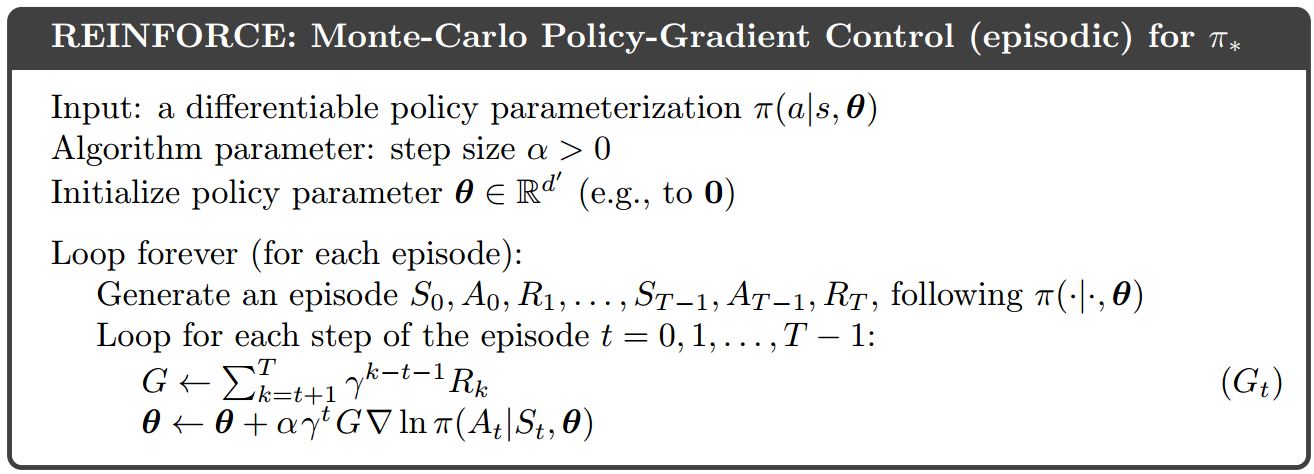
\includegraphics[scale = 0.3]{reinforce_algo.png}}
\end{minipage}
\caption{\footnotesize{\textbf{The REINFORCE: Monte Carlo policy gradient}}}
\label{fig: reinforce_algo}
\end{figure}
Therefore, we have the \textbf{REINFORCE update:}
\begin{align}
\mb{\theta}_{t+1} &\leftarrow \mb{\theta}_{t} + \alpha \;G_{t}\grad{\mb{\theta}}{\log\pi(A_{t}|S_{t}, \mb{\theta})}, \label{eqn: reinforce_update}
\end{align} where $G_{t}$ is the sample returns under the policy $\pi$ following the sequence $(S_{t}, A_{t}, \ldots)$ in an episode.  REINFORCE is a \underline{\textbf{Monte Carlo policy gradient method}}, since the algorithm will not update the policy until the \textbf{end of each episode}, in order to obtain the sample return $G_{t}$. Figure \ref{fig: reinforce_algo} shows the \textbf{REINFORCE as Monte Carlo policy gradient method} for \emph{episodic task}.

Like many Monte Carlo methods, REINFORCE is \textbf{unbiased} but have \textbf{high variance} and \textbf{slow learning}. As a stochastic gradient method, REINFORCE has good \emph{theoretical \textbf{convergence} properties}. By construction, the expected update over an episode is in the same direction as the performance gradient. This \emph{assures an improvement} in expected performance for sufficiently small $\alpha$, and convergence to a \textbf{local optimum} under standard stochastic approximation conditions for decreasing $\alpha$.  

\begin{figure}
\begin{minipage}[t]{1\linewidth}
  \centering
  \centerline{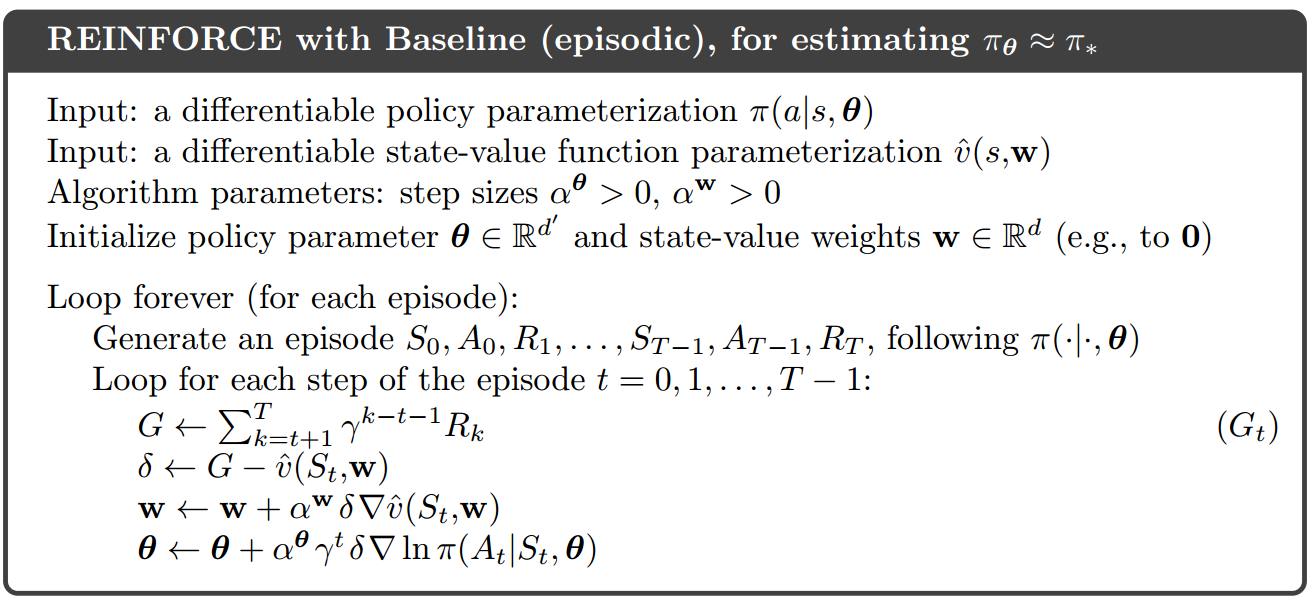
\includegraphics[scale = 0.3]{reinforce_baseline_algo.png}}
\end{minipage}
\caption{\footnotesize{\textbf{The REINFORCE with value function baseline: Monte Carlo policy gradient}}}
\label{fig: reinforce_baseline_algo}
\end{figure}

The REINFORCE update has some appealing properties: Each increment is proportional to the product of a return $G_t$ and a vector, the gradient of the log-probability of taking the sample action. This vector is the direction in paramete space that \textbf{\emph{most} increases} the \emph{\textbf{probability} of \textbf{repeating} the action $A_t$ on \textbf{future} visits} to state $S_t$. The update increases the parameter vector in this direction \textbf{proportional to the return}, and \textbf{inversely proportional to the action probability}. The former makes sense because it causes the parameter to move most in the directions that \emph{favor actions}
that yield the \underline{highest return}. The latter makes sense because otherwise actions that are selected \underline{frequently} are \underline{at an advantage} (the updates will be more often in their direction) and might win out even if they do not yield the highest return.


\subsection{REINFORCE with baseline}
The policy gradient theorem can be generalized to include arbitrary baseline $b(\mb{s})$
\begin{align*}
\grad{\mb{\theta}}{\cR(\mb{\theta})} &\propto \sum_{s}\mu_{\pi(\mb{\theta})}(s)\sum_{a}\grad{\mb{\theta}}{\pi(a |\mb{s}, \mb{\theta})}\paren{q_{\pi}(\mb{s}, a) - b(\mb{s})}
\end{align*} The equation holds since $b(\mb{s})\sum_{a}\grad{\mb{\theta}}{\pi(a |\mb{s}, \mb{\theta})} = 0$. Thus the \textbf{REINFORCE-with-baseline} update
\begin{align}
\mb{\theta}_{t+1} &\leftarrow \mb{\theta}_{t} + \alpha \;(G_{t}-b(S_t))\grad{\mb{\theta}}{\log\pi(A_{t}|S_{t}, \mb{\theta})}, \label{eqn: reinforce_update_w_baseline}
\end{align} In general, the baseline leaves the expected value of the update unchanged, but the \textbf{variance will be reduced} significantly. A natural choice of baseline function is the approximate value function $\hat{v}(S_t, \mb{w}_t)$, whose function parameter is updated using Monte Carlo prediction.  Figure \ref{fig: reinforce_baseline_algo} describes the REINFORCE with value function estimate as baseline. 

Note that although the REINFORCE-with-baseline method learns both a policy and a state-value function, we do not consider it to be an actor–critic method because its \emph{state-value function} is used only as a \emph{\textbf{baseline}}, not as a critic. That is, it is not used for bootstrapping that updates the value estimate for a state from the estimated values of subsequent states. This is a useful distinction, for only through bootstrapping do we introduce \textbf{bias} and an \textbf{asymptotic dependence}
on the quality of the function approximation. 


\section{Actor-Critic Methods}
The idea behind the Actor-Critic Methods is to use \textbf{boostrapping} which estimates the value estimate for current state based on value estimate of its successor states. The \textbf{TD error} is used for both \textbf{\emph{value estimation}} (prediction) and \emph{\textbf{policy gradient}} (control). By introducing bias and an \textbf{asymptotic dependence} on the quality of the \emph{function approximation}, Actor-Critic Methods learn policy faster with less variance. 
\begin{figure}
\begin{minipage}[t]{1\linewidth}
  \centering
  \centerline{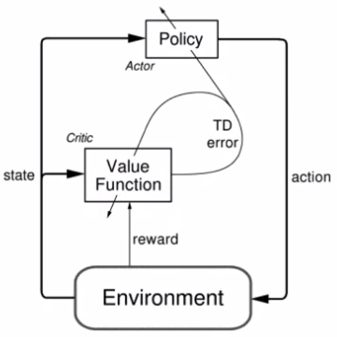
\includegraphics[scale = 0.5]{actor_critic.png}}
\end{minipage}
\caption{\footnotesize{\textbf{The Actor-Critic methods}}}
\label{fig: actor_critic}
\end{figure}
First consider \textbf{one-step actor–critic methods}. There are two roles for the agent:
\begin{itemize}
\item \textbf{Actor}: the role of an \textbf{actor} is to \textbf{\emph{update the policy distribution}} via policy gradient algorithm. The analog of the TD methods introduced, we choose to replace the sample return in the \emph{REINFORCE-with-baseline} with  boostrapping $\hat{G}_{t} = R_{t+1} + \gamma\hat{v}(S_{t+1}, \mb{w}_t )$. The updates for \emph{actor} is shown below
\begin{align}
\mb{\theta}_{t+1} &\leftarrow \mb{\theta}_{t} + \alpha_{\mb{\theta}} \;(\hat{G}_{t}-\hat{v}(S_{t}, \mb{w}_t ))\grad{\mb{\theta}}{\log\pi(A_{t}|S_{t}, \mb{\theta})} \nonumber\\
&= \mb{\theta}_{t} +  \alpha_{\mb{\theta}} \;(R_{t+1} + \gamma\hat{v}(S_{t+1}, \mb{w}_t ) -  \hat{v}(S_{t}, \mb{w}_t ))\grad{\mb{\theta}}{\log\pi(A_{t}|S_{t}, \mb{\theta})}  \nonumber\\
&= \mb{\theta}_{t} + \alpha_{\mb{\theta}}  \;\underline{\delta_t}\; \grad{\mb{\theta}}{\log\pi(A_{t}|S_{t}, \mb{\theta})} \label{eqn: actor_update}
\end{align} where 
\begin{align*}
\delta_{t}&= R_{t+1} + \gamma \hat{v}(S_{t+1}, \mb{w}_{t}) - \hat{v}(S_{t}, \mb{w}_{t})
\end{align*}
 is the \textbf{TD error}. When TD error is positive, the selected action resulted in a higher value than expected, which is desireable. \emph{ The actor updates the policy distribution \textbf{based on  value function provided by critic}}.

\item \textbf{Critic}: Given the learned policy $\pi(a|\mb{s}, \mb{\theta})$, the role of a \textbf{critic} is to \textbf{\emph{evalute} the \emph{value} of the policy} and used it as a \textbf{feedback} for actor's performance. As shown in Figure \ref{fig: actor_critic}, the same TD error $\delta_t$ is used by \textbf{semi-gradient methods} (e.g. TD(0)) for function apprximation.
\begin{align}
\mb{w}_{t+1} &\leftarrow  \mb{w}_{t} + \alpha_{\mb{w}} \;\underline{\delta_{t}}\; \grad{\mb{w}}{\hat{v}(S_{t}, \mb{w}_{t})}  \label{eqn: critic_update}
\end{align} As oppose to actor which maximize the value by improving the policy, the update \eqref{eqn: critic_update} will adjust the value function to \textbf{match} the \emph{\textbf{target value}}, i.e. moving in direction to minimize the Mean Squared Value Error.
\begin{figure}
\begin{minipage}[t]{1\linewidth}
  \centering
  \centerline{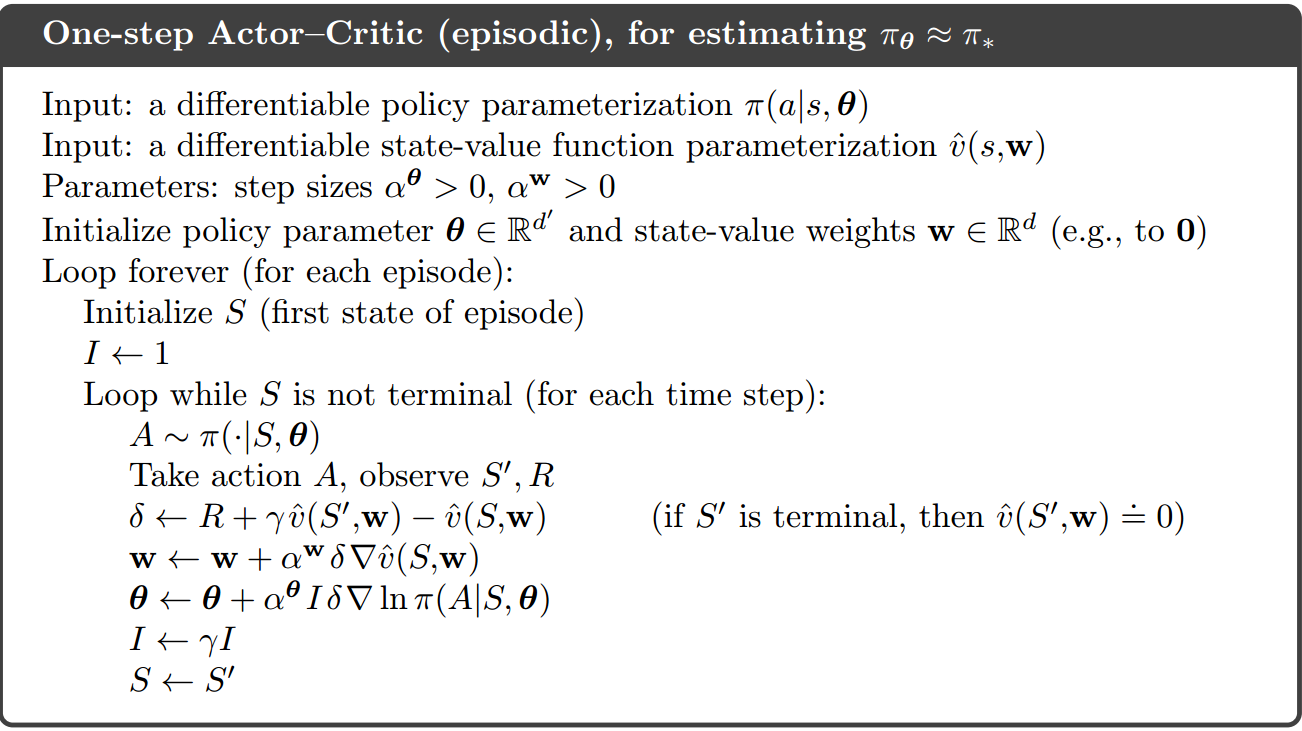
\includegraphics[scale = 0.3]{actor_critic_algo.png}}
\end{minipage}
\caption{\footnotesize{\textbf{The Actor-Critic methods}}}
\label{fig: actor_critic_algo}
\end{figure}
\end{itemize} Figure \ref{fig: actor_critic_algo} shows the \emph{actor-critic algorithm with one-step TD updates}. Since the algorithm use the value function estimate as a baseline, it is also called the \textbf{Advantage Actor Critic (A2C)}.



Note that we can replace the state-value function with the  \textbf{action-value function}, which includes TD error for SARSA, Q-learning and Expected SARSA. 
\begin{align*}
\grad{\mb{\theta}}{\cR} &= \E{\pi}{q_{\pi}(S_{t}, A_{t}) \frac{\grad{\mb{\theta}}{\pi(A_{t}|S_{t}, \mb{\theta})}}{\pi(A_{t}|S_{t}, \mb{\theta})} }
\end{align*} In the \textbf{Q Actor Critic}, for the actor, the policy gradient update is the stochastic gradient ascent (use sample action in \eqref{eqn: policy_grad_sga}) as below: 
\begin{align}
\mb{\theta}_{t+1} &\leftarrow  \mb{\theta}_{t} + \alpha_{\mb{\theta}}\;\hat{q}(S_{t}, A_{t}, \mb{w}_{t}) \;\grad{\mb{\theta}}{\log\pi(A_{t}|S_{t}, \mb{\theta})} \nonumber
\end{align} and for critic, the semi-gradient methods for value function update as below:
\begin{align}
\mb{w}_{t+1} &\leftarrow  \mb{w}_{t} + \alpha_{\mb{w}}\, \delta_{t}\,\grad{\mb{w}}{\hat{q}(S_{t}, A_{t}, \mb{w}_{t})}  \nonumber
\end{align} where the TD error $\delta_t$ are defined as below:  
\begin{align}
\text{  \textbf{SARSA} }\quad \delta_{t}&:=\brac{R_{t+1} + \gamma \hat{q}(S_{t+1}, A_{t+1}, \mb{w}_{t}) - \hat{q}(S_{t}, A_{t}, \mb{w}_{t})}  \label{eqn: semi_grad_sarsa}\\
\text{  \textbf{Q-Learning} }\quad \delta_{t}&:=\brac{R_{t+1} + \gamma \max_{a'}\hat{q}(S_{t+1}, a', \mb{w}_{t}) - \hat{q}(S_{t}, A_{t}, \mb{w}_{t})}   \label{eqn: semi_grad_q_learning}\\
 \text{  \textbf{Expected Sarsa} }\quad \delta_{t} &= \brac{R_{t+1} +\gamma\sum_{a'}\pi(a'|S_{t+1})\hat{q}(S_{t+1}, a', \mb{w}_{t}) - \hat{q}(S_{t}, A_{t}, \mb{w}_{t})}  \label{eqn: semi_grad_exp_sarsa} 
\end{align}





\newpage
\bibliographystyle{plainnat}
\bibliography{reference.bib}
\end{document}